% -*- mode:flyspell; mode:latex  -*-

%%% Local Variables:
%%% TeX-master: "mu2e-36575"
%%% End:

%%%%%%%%%%%%%%%%%%%%%%%%%%%%%%%%%%%%%%%%%%%%%%%%%%%%%%%%%%%%%%%%%%%%%%%%%%%%% 
\section{Track momentum corrections}

The mean value of the reconstructed track momentum extrapolated to the tracker entrance is
slightly lower than the true MC momentum of the corresponding MC particle.
The offset is of the order of 30 keV/c and slightly different the track fits with different
ambiguity resolvers.
We correct the reconstructed momenta of PAR tracks by 34 keV/c , and DAR tracks - by 30 keV/c.

\begin{figure}
\hspace{-1.4in}
\begin{tikzpicture}
  \node[anchor=south west,inner sep=0] at (0,0.) {
    % \node[shift={(0 cm,0.cm)},inner sep=0,rotate={90}] at (0,0) {}
    % \makebox[\textwidth][c] {
      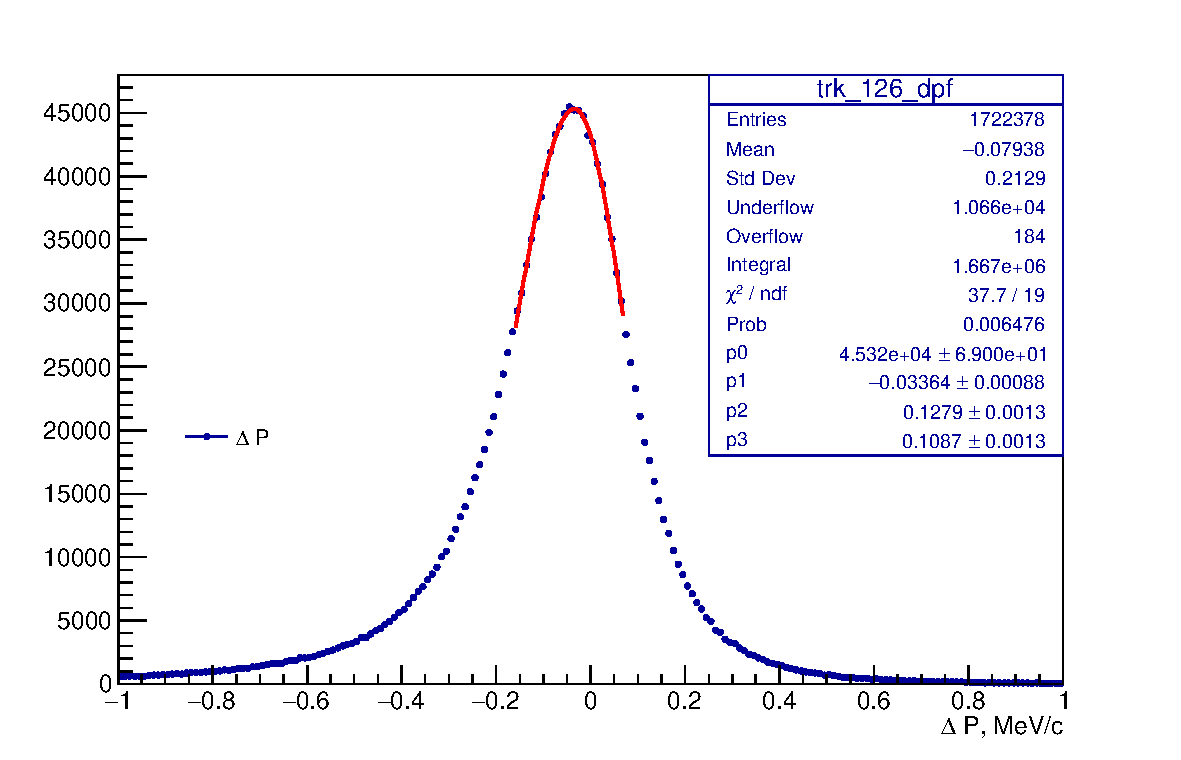
\includegraphics[width=0.80\textwidth]{figures/pdf/figure_00112_fele2s51b1_track_comp_ffff_1070_nocorr_trk_126_dpf}
    %}
  };
  \node[anchor=south west,inner sep=0] at (10,0.) {
    % \node[shift={(0 cm,0.cm)},inner sep=0,rotate={90}] at (0,0) {}
    % \makebox[\textwidth][c] {
      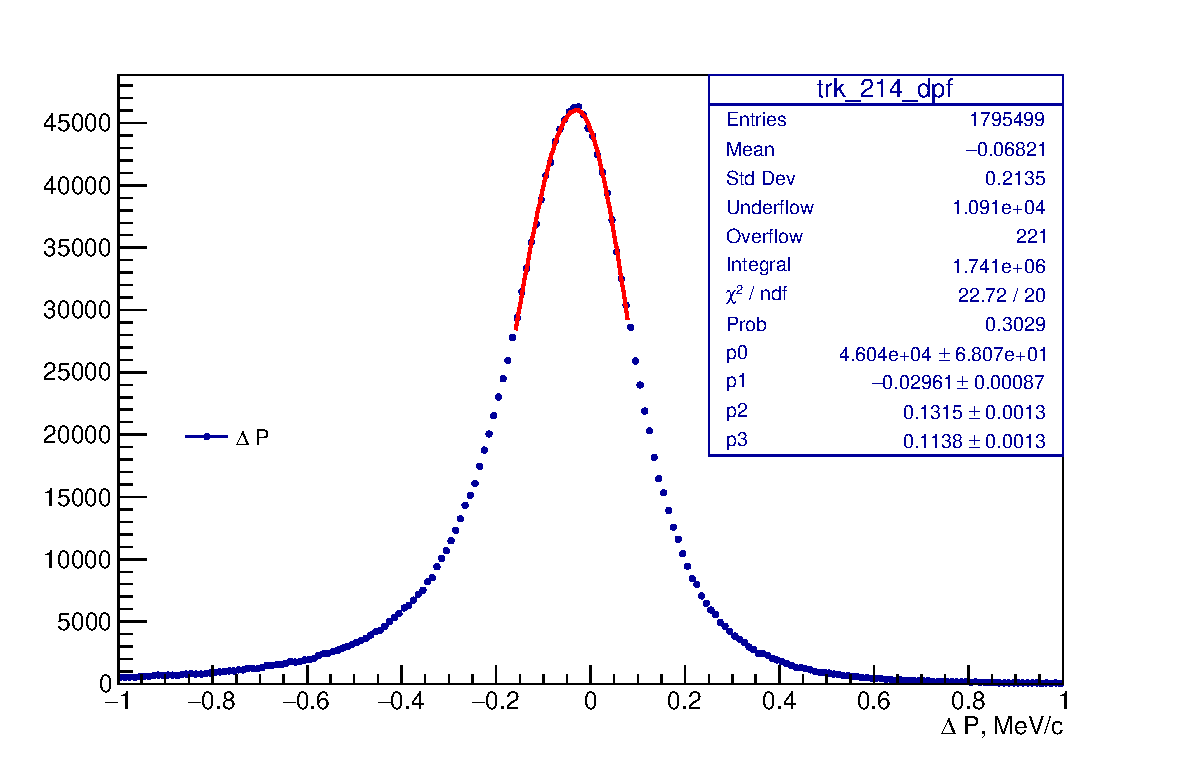
\includegraphics[width=0.80\textwidth]{figures/pdf/figure_00113_fele2s51b1_track_comp_ffff_1070_nocorr_trk_214_dpf}
    %}
  };
  % \node [text width=6cm, scale=0.8] at (4.5,6.4) {mu2e-18894 by Kevin Lynch and Jim Popp};
\end{tikzpicture}

\caption{
  \label{fig:sindrum_ii_fig_08_fit} 
  $\Delta P$ distributions at the tracker front for PAR (left) and DAR (right) tracks. The distributions  
  are fit with the asymmetric ($\sigma_{left} \ne \sigma_{right}$) gaussian function. Peak positions are used
  to correct the reconstructed  momenta of the tracks coming of the respective fits.
}
\end{figure}

%%%%%%%%%%%%%%%%%%%%%%%%%%%%%%%%%%%%%%%%%%%%%%%%%%%%%%%%%%%%%%%%%%%%%%%%%%%%% 
\section{Track Selections}

Selection of correctly reconstructed tracks plays a critical role in the search.
In the Mu2e offline, there are two track fitters which correspond to two different
hit ambiguity resolvers. An ANN-based training has been performed only for one of them,
so-called ``panel-based ambiguity resolver''.

We performed a similar training for the output of the track fits using the doublet-based
ambiguity resolver.

Following \cite{MU2E_4595_ANN_TRAINING}, we used ROOT TMVA package to train a MLP ANN
with 8 input variables and one hidden layer. The following eight variables were used as inputs:

\begin{itemize}
\item
  {\bf na }: number of ``active'' hits remaining on the track after the Kalman fit
\item
  {\bf  nafract} = na/nhits , ratio of the number of active hits to the total number of hits
  (after the seed fit)
\item
  $log_{10}{fcons}$ : {\bf fcons}, or fit consistency is a probability-minded derivative
  from the track fit $\chi^2$. Logarithm of it it taken from the numerical considerations
\item
  {\bf momerr}: uncertainty on the reconstructed track momentum, returned by the fitter
\item
  {\bf t0err} : uncertainty on the reconstructed track time, T0, returned by the fitter
\item
  {\bf fda} : = Nd/Na, fraction of ``doublet'' active hits
\item
  {\bf fza } : = Nza/Na, fraction of activev hits with undefined drift direction
\item
  {\bf fma } : {\bf \red to be clarified}
\end{itemize}

Training was aimed to optimize separation of electron tracks reconstructed correctly, 
with $\Delta{P} = |P_{reco}-P_{true}| < 0.25$ MeV/c, or with momenta reconstructed approximately
within $2\sigma$ from the true value, from tracks reconstructed
with $\Delta{P} > 0.7$ MeV/c, or , approximately, $5\sigma$ above the true value.

Comparison between $P_{true}$ and $P_{reco}$ was performed in a  plane corresponding to the tracker front.

Tracks used for the ANN training were required to have |D0| < 100 mm and 0.5 < \tandip < 1 is. 

To choose between the PAR-based and DAR-based fitters, we compared performance of the
trained DAR ANN to the performance of the PAR ANN.

The results are shown in Figure ..... .
Using the CD3 choice of the signal region , 103.85 < p < 104.90 MeV/c, we compared the
CE reconstruction efficiency of the two methods vs the expected DIO background.

Figure \ref{fig:ann_operational_point_choice} shows the result.

Use of the DAR track fits allows to increase acceptance by 4-5\%, while keeping the expected
background below the level corresponding to PAR fits.

The operational point corresponds to the cut on the output of DAR ANN $S_{DAR} > 0.2$.

\begin{figure}
\begin{tikzpicture}
  \node[anchor=south west,inner sep=0] at (0,0.) {
    % \node[shift={(0 cm,0.cm)},inner sep=0,rotate={90}] at (0,0) {}
    \makebox[\textwidth][c] {
      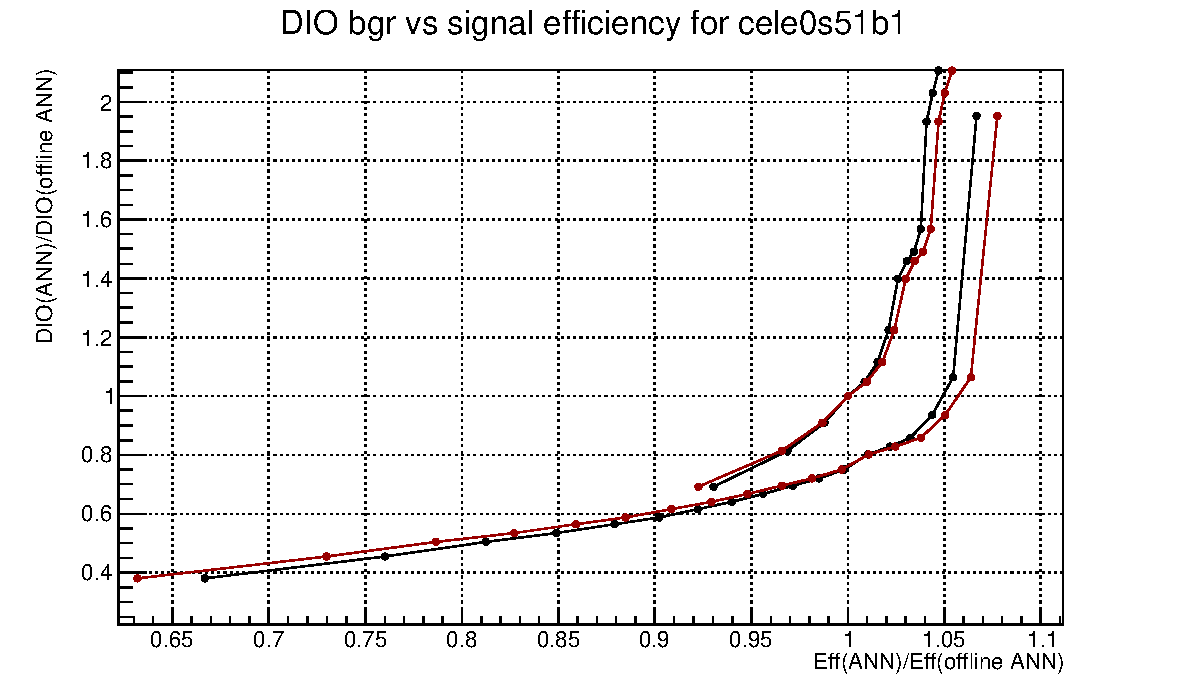
\includegraphics[width=0.99\textwidth]{figures/pdf/ann_operational_point_choice}
    }
  };
  % \node [text width=6cm, scale=0.8] at (4.5,6.4) {mu2e-18894 by Kevin Lynch and Jim Popp};
\end{tikzpicture}
% \captionof{figure} {
\caption{
  \label{fig:ann_operational_point_choice}
  Choice of the ANN operational point. background numbers - from fele2s51b1,
  signal efficiency: black points: cele0s51b1; Red: cele0s51b2;
  Compared to PAR track selection $S_{PAR} > 0.8$, selecting DAR tracks with $S_{DAR} > 0.2$ 
  improves acceptance in the CD3 signal region of [103.85,104.90] by 4-5\%, 
  while keeping the DIO background at a lower level.
  {\color{red} {\bf *** update caption **}}
}
\end{figure}

Figure \ref{fig:dar_vs_par_ann} compares distributions of the track momentum resolution for DAR ANN-based track
selections and PAR ANN-based track selection. For the PAR fit, the track selection corresponding to For DAR fits, 
we show two operational points corresponding to the same efficiency and the same expected DIO background.

\begin{figure}
\hspace{-1.4in}
\begin{tikzpicture}
  \node[anchor=south west,inner sep=0] at (0,0.) {
    % \node[shift={(0 cm,0.cm)},inner sep=0,rotate={90}] at (0,0) {}
    % \makebox[\textwidth][c] {
    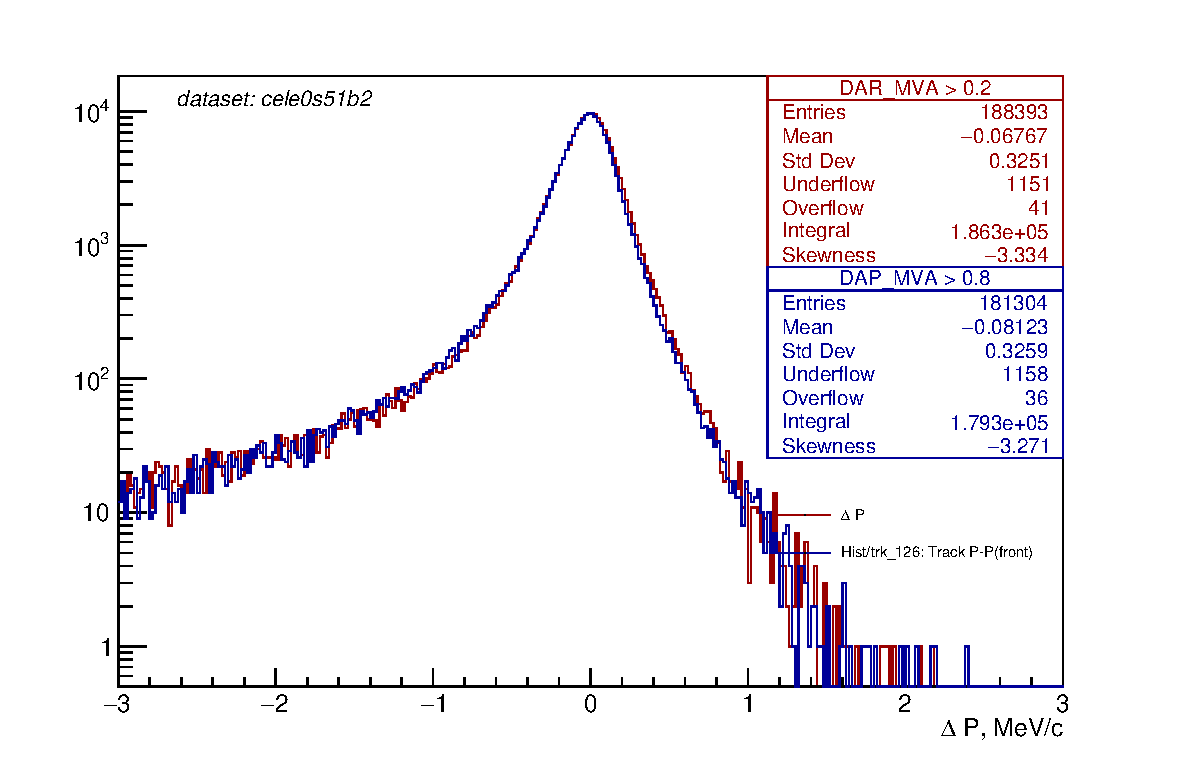
\includegraphics[width=0.80\textwidth]{figures/pdf/figure_00114_cele0s51b2_track_comp_ffff_1070_trk_214_vs_126_dpf}
    % }
  };
  \node[anchor=south west,inner sep=0] at (10,0.) {
    % \node[shift={(0 cm,0.cm)},inner sep=0,rotate={90}] at (0,0) {}
    % \makebox[\textwidth][c] {
    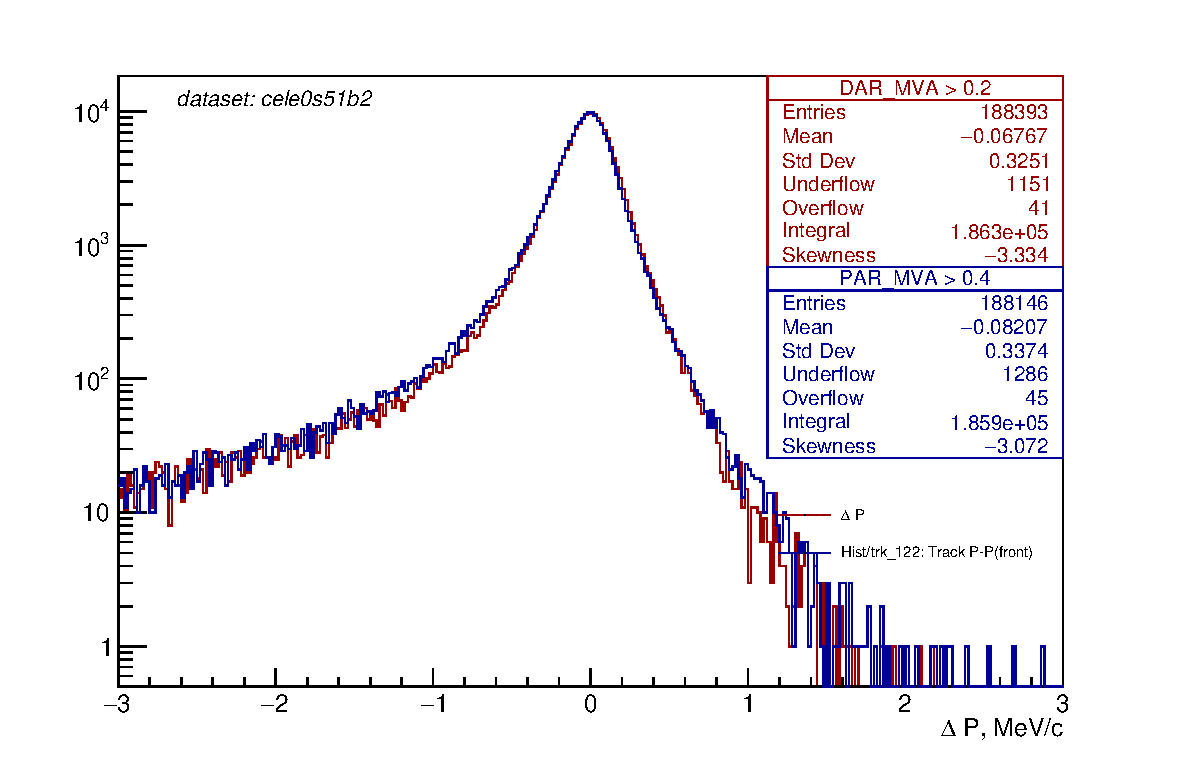
\includegraphics[width=0.80\textwidth]{figures/pdf/figure_00116_cele0s51b2_track_comp_ffff_1070_trk_214_vs_122_dpf}
    % }
  };
  % \node [text width=6cm, scale=0.8] at (4.5,6.4) {mu2e-18894 by Kevin Lynch and Jim Popp};
\end{tikzpicture}
% \captionof{figure} {
\caption{
  \label{fig:dar_vs_par_ann}
  track momentum resolution at the tracker front. 
  DAR vs PAR track selection efficiency for two operational points, left: DAR and PAR selections correspond to the same background, 
  right: DAR and PAR selections correspond to the same efficiency. The right-hand tail give the measure of quality 
}
\end{figure}

Improvements in the track reconstruction resulted in a significantly better separation between the two classes of tracks.
Shown in Figure \ref{fig:dio_delta_p_1036_1050} is the $\Delta{P}$ distribution for the simulated DIO electrons.
with momenta reconstructed in the region [103.6, 105.0] MeV/c.
Fraction of tracks with significantly mis-reconstructed momenta, $\Delta{P} > 0.5$ MeV, is about 0.23.
about 50\% lower than 0.355, estimated in the same momentum window in \cite{MU2E_4595_ANN_TRAINING}..

\begin{figure}
  \begin{tikzpicture}
    \node[anchor=south west,inner sep=0] at (0,0.) {
      % \node[shift={(0 cm,0.cm)},inner sep=0,rotate={90}] at (0,0) {}
      \makebox[\textwidth][c] {
        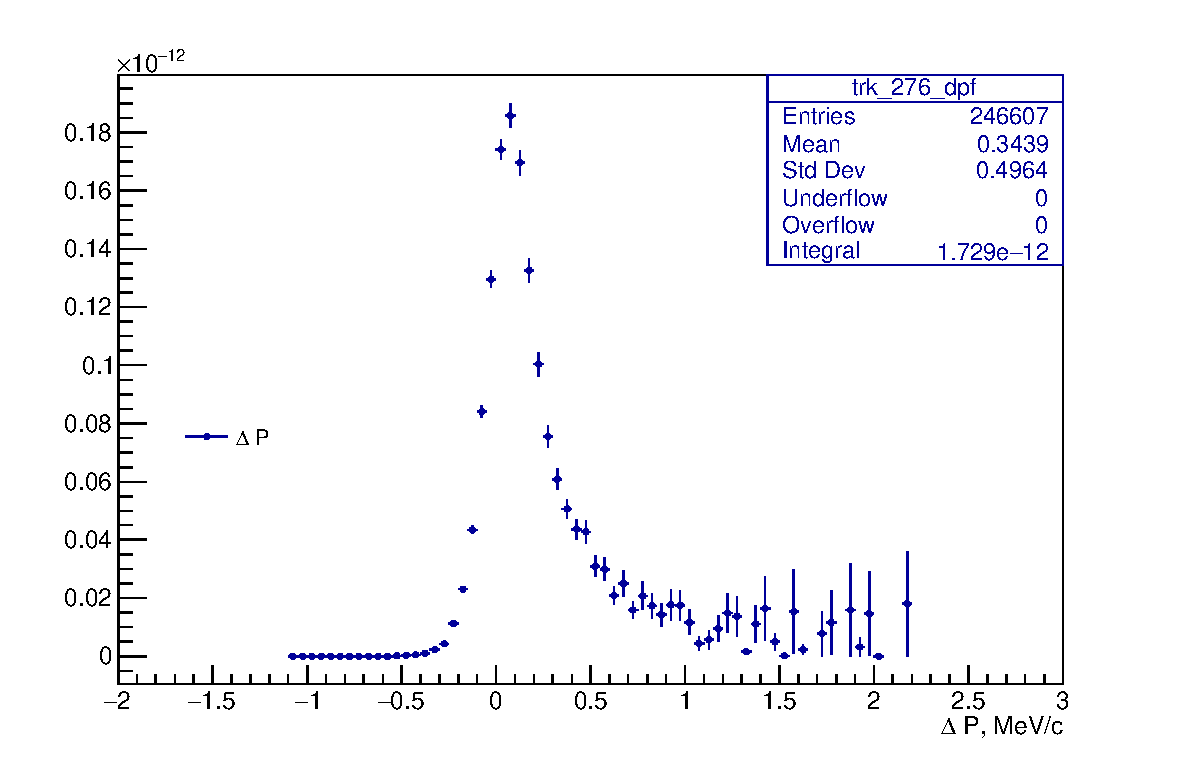
\includegraphics[width=0.99\textwidth]{figures/pdf/figure_00111_fele2s51b1_track_comp_ffff_1070_trk_276_dpf}
      }
    };
    % \node [text width=6cm, scale=0.8] at (4.5,6.4) {mu2e-18894 by Kevin Lynch and Jim Popp};
  \end{tikzpicture}
  % \captionof{figure} {
  \caption{
    \label{fig:dio_delta_p_1036_1050} 
    $\Delta P ~=~ P_{reco} -P_{true}$ distribution for simulated DIO background in the region [103.6,105.0] MeV.
    77.2\% of reconstructed events in this region are expected to have $\Delta P < 0.5$ MeV/c
  }
\end{figure}

As a cross-check, we trained a BDT-based TMVA classifier. Similar to \cite{MU2E_33150_ANN_TRAINING},
we found that the ANN performed slightly better, so current analysis uses an ANN-based track
quality selection.

To explore the parameter space, a similar ANN has been trained to discriminate the tracks reconstructed
with $\Delta{P} < 0.25$ MeV/c from tracks with $\Delta{P} > 0.6$ MeV/c. No improvement in the DIO
suppression in the region [103.85, 104.9] MeV/c was observed. 

Continuing the phase space exploration, we trained an similar ANN with the bato discriminate the tracks for
$\Delta{P} < 0.25$ MeV/c from tracks with $\Delta{P} > 0.6$ MeV/c. No improvement in the DIO
suppression in the region [103.85, 104.9] MeV/c was observed. 

%%%%%%%%%%%%%%%%%%%%%%%%%%%%%%%%%%%%%%%%%%%%%%%%%%%%%%%%%%%%%%%%%%%%%%%%%%%%%%
\subsection{Final track quality selections}

The finalized track selection includes three cuts. The track impact parameter cut selects tracks consistent 
with coming from the stopping target, the track $\tan\lambda$ cut, in essense, is an anti-cosmics cut, and 
its final value needs to be optimized. The cut on the ANN output, or score, variable selects
well reconstucted tracks.

\begin{table}[h!]
  \begin{center}
    \begin{tabular}{l|c|c} % <-- Changed to S here.
      \textbf{Cut variable} & \textbf{Cut value} & \textbf{``N-1'' Efficiency for CE}\\
      \hline
      track impact parameter,  D0 & | D0 | < 100 mm           &   0.990    \\
      track dip angle, \tandip    & $ 0.5< \tan \lambda < 1.$ &   0.909    \\
      track quality ANN score, $S_{TRQ}$      & $S_{TRQ} > 0.2$            &   0.901    \\
    \end{tabular}
  \end{center}
  \caption{
    \label{tab:trq_cuts}
    Final Track quality selection
  }
\end{table}

Table \ref{table:ce_trq_efficiency_vs_pileup} benchmarks the selection efficiencies for fits using two different
anbiguity resolvers

\begin{table}[h!]
  \begin{center}
    \caption{Efficiency for different levels of pile-up occupancy}
    \label{tab:table1}
    \begin{tabular}{l|c|c|c} % <-- Changed to S here.
      \textbf{pileup}    & Eff DAR &  Efficiency PAR  &  DAR/PAR   \\
      \hline                                                           
      CE                 &  0.152  &   0.149          &  1.02      \\
      CE+1-batch pileup  &  0.152  &   0.146          &  1.04      \\
      CE+2-batch pileup  &  0.149  &   0.143          &  1.04      \\
    \end{tabular}
  \end{center}
  \caption{
    \label{table:ce_trq_efficiency_vs_pileup_1} 
    conversion electron (CE) track selection efficiency for different levels of pileup and momentum window [103,105.0]  
    and T0 > 700 ns
  }
\end{table}


% PAR 1b:107810

\begin{table}[h!]
  \label{table:ce_trq_efficiency_vs_pileup_2} 
  \begin{center}
    \begin{tabular}{l|c|c|c} % <
      \textbf{pileup}    & Eff DAR &  Efficiency PAR  &  DAR/PAR   \\
      \hline                                                           
      CE                 &  0.111  &   0.104          &  1.07      \\
      CE+1-batch pileup  &  0.113  &   0.108          &  1.05      \\
      CE+2-batch pileup  &  0.111  &   0.105          &  1.05      \\
    \end{tabular}
  \end{center}
  \caption{
    conversion electron (CE) track selection efficiency for different levels of pileup and momentum window [103.85,105.0] 
    and T0 > 700 ns
  }
\end{table}





